\documentclass[border=4pt]{standalone}
\usepackage{tikz}
\usetikzlibrary{calc}
\usepackage{pgfplots}
\pgfplotsset{compat=1.18}
\usepackage{amsmath}

\begin{document}
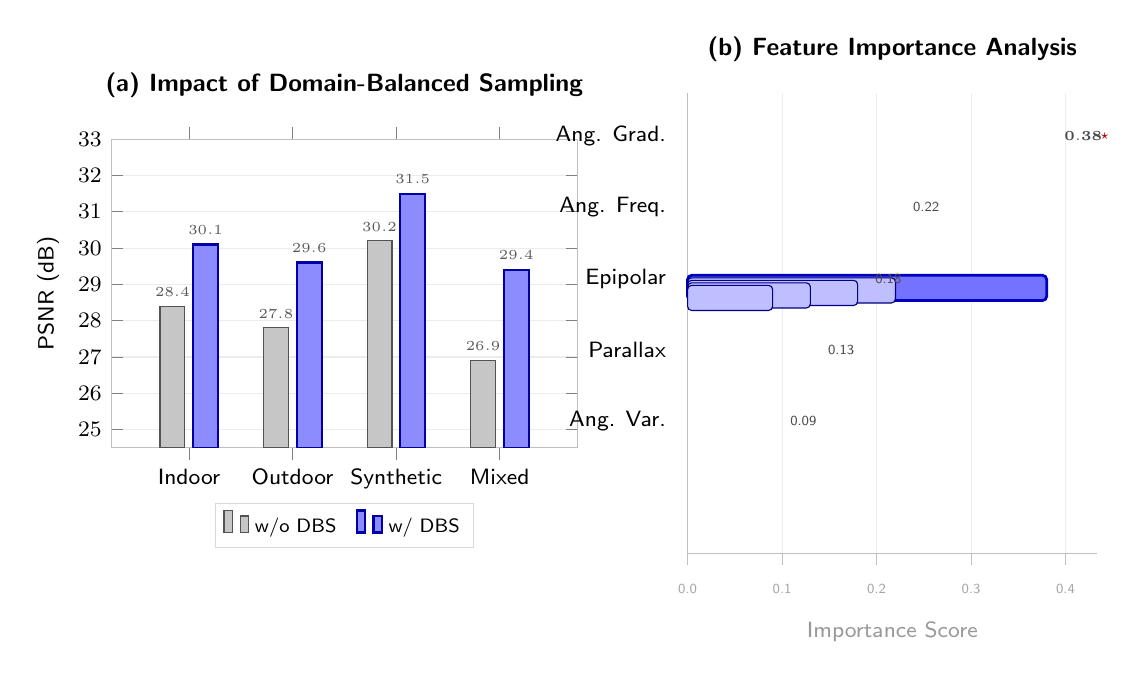
\begin{tikzpicture}

% ===== (a) Grouped bar chart =====
\begin{axis}[
    name=plotA,
    ybar=3pt,
    bar width=9pt,
    width=7.5cm,
    height=5.5cm,
    symbolic x coords={Indoor,Outdoor,Synthetic,Mixed},
    xtick=data,
    x tick label style={font=\sffamily\footnotesize},
    ylabel={PSNR (dB)},
    ylabel style={font=\sffamily\footnotesize},
    ymin=24.5,
    ymax=33,
    ytick={25,26,27,28,29,30,31,32,33},
    y tick label style={font=\sffamily\footnotesize},
    legend style={
        at={(0.5,-0.18)},
        anchor=north,
        legend columns=2,
        font=\sffamily\scriptsize,
        draw=gray!30,
        /tikz/every even column/.append style={column sep=5pt},
    },
    enlarge x limits=0.25,
    nodes near coords,
    nodes near coords style={font=\tiny\sffamily, color=black!65,
      /pgf/number format/.cd, fixed, precision=1},
    axis line style={gray!50},
    ymajorgrids=true,
    grid style={gray!15, thin},
    title style={font=\sffamily\small\bfseries, at={(0.5,1.05)}},
    title={(a) Impact of Domain-Balanced Sampling},
]
\addplot[fill=gray!45, draw=gray!65!black]
    coordinates {(Indoor,28.4) (Outdoor,27.8) (Synthetic,30.2) (Mixed,26.9)};
\addplot[fill=blue!45, draw=blue!65!black, line width=0.8pt]
    coordinates {(Indoor,30.1) (Outdoor,29.6) (Synthetic,31.5) (Mixed,29.4)};
\legend{w/o DBS, w/ DBS}
\end{axis}

% ===== (b) Feature importance - manual horizontal bars =====
\begin{scope}[shift={($(plotA.east)+(1.4,0)$)}]

% Title
\node[font=\sffamily\small\bfseries] at (2.6,3.1) {(b) Feature Importance Analysis};

% Parameters
\def\bh{0.32cm}
\def\yscale{0.95}

% Grid lines
\foreach \x/\v in {0/0.0, 1.2/0.1, 2.4/0.2, 3.6/0.3, 4.8/0.4} {
    \draw[gray!15, thin] (\x,-3.3) -- (\x,2.55);
}

% Axis lines
\draw[gray!50] (0,-3.3) -- (0,2.55);
\draw[gray!50] (0,-3.3) -- (5.2,-3.3);

% X-axis ticks
\foreach \x/\v in {0/0.0, 1.2/0.1, 2.4/0.2, 3.6/0.3, 4.8/0.4} {
    \draw[gray!50] (\x,-3.3) -- (\x,-3.45);
    \node[font=\tiny\sffamily, gray!70] at (\x,-3.75) {\v};
}
\node[font=\sffamily\footnotesize, gray!80] at (2.6,-4.3) {Importance Score};

% Bar: Ang. Grad. (highlighted, dominant)
\pgfmathsetmacro{\bw}{0.38/0.4*4.8}
\fill[blue!55, draw=blue!75!black, line width=1pt, rounded corners=1.5pt]
    (0, {2.1*\yscale-\bh/2}) rectangle ({\bw}, {2.1*\yscale+\bh/2});
\node[font=\sffamily\footnotesize, anchor=east] at (-0.15, {2.1*\yscale}) {Ang. Grad.};
\node[font=\tiny\sffamily, black!70, anchor=west] at ({\bw+0.1}, {2.1*\yscale}) {$\mathbf{0.38}$};
\node[font=\tiny\sffamily, red!70!black, anchor=west] at ({\bw+0.55}, {2.1*\yscale}) {$\star$};

% Bar: Ang. Freq.
\pgfmathsetmacro{\bw}{0.22/0.4*4.8}
\fill[blue!25, draw=blue!50!black, rounded corners=1.5pt]
    (0, {1.15*\yscale-\bh/2}) rectangle ({\bw}, {1.15*\yscale+\bh/2});
\node[font=\sffamily\footnotesize, anchor=east] at (-0.15, {1.15*\yscale}) {Ang. Freq.};
\node[font=\tiny\sffamily, black!70, anchor=west] at ({\bw+0.1}, {1.15*\yscale}) {0.22};

% Bar: Epipolar
\pgfmathsetmacro{\bw}{0.18/0.4*4.8}
\fill[blue!25, draw=blue!50!black, rounded corners=1.5pt]
    (0, {0.2*\yscale-\bh/2}) rectangle ({\bw}, {0.2*\yscale+\bh/2});
\node[font=\sffamily\footnotesize, anchor=east] at (-0.15, {0.2*\yscale}) {Epipolar};
\node[font=\tiny\sffamily, black!70, anchor=west] at ({\bw+0.1}, {0.2*\yscale}) {0.18};

% Bar: Parallax
\pgfmathsetmacro{\bw}{0.13/0.4*4.8}
\fill[blue!25, draw=blue!50!black, rounded corners=1.5pt]
    (0, {-0.75*\yscale-\bh/2}) rectangle ({\bw}, {-0.75*\yscale+\bh/2});
\node[font=\sffamily\footnotesize, anchor=east] at (-0.15, {-0.75*\yscale}) {Parallax};
\node[font=\tiny\sffamily, black!70, anchor=west] at ({\bw+0.1}, {-0.75*\yscale}) {0.13};

% Bar: Ang. Var.
\pgfmathsetmacro{\bw}{0.09/0.4*4.8}
\fill[blue!25, draw=blue!50!black, rounded corners=1.5pt]
    (0, {-1.7*\yscale-\bh/2}) rectangle ({\bw}, {-1.7*\yscale+\bh/2});
\node[font=\sffamily\footnotesize, anchor=east] at (-0.15, {-1.7*\yscale}) {Ang. Var.};
\node[font=\tiny\sffamily, black!70, anchor=west] at ({\bw+0.1}, {-1.7*\yscale}) {0.09};

\end{scope}

\end{tikzpicture}
\end{document}